%_____________________________________________________________________________________________ 
% LATEX Template: Department of Comp/IT BTech Project Reports
% Main Report
% Sun Apr 1 20:40:00 IST 2011
% 
%_____________________________________________________________________________________________ 

\documentclass[a4paper,14pt,onecolumn]{report}

%_____________________________________________________________________________________________ 
% Inclusion of Required Packages
% TODO: \usepackage{graphicx} required
%
%_____________________________________________________________________________________________ 
\usepackage[dvips]{graphics}
\usepackage{color}
\usepackage{epsfig}
\usepackage[strings]{underscore}
\usepackage{titlesec}
\usepackage{url}
\usepackage{setspace}
\usepackage{float}
\titleformat{\chapter}{}{}{0em}{\bf\LARGE}
\titlespacing*{\chapter}{0pt}{10pt}{20pt}
%_____________________________________________________________________________________________ 
% Page Layout
%_____________________________________________________________________________________________ 
\setlength{\textwidth}{6.27in}
\setlength{\textheight}{9.69in}
\setlength{\topmargin}{0.0in}
\setlength{\oddsidemargin}{0.0in}			% Customisable
\setlength{\headheight}{0.0in}
\setlength{\headsep}{0.0in}
\setlength{\topskip}{0.0in}
%_____________________________________________________________________________________________ 
% Font Definition
%_____________________________________________________________________________________________ 
\fontencoding{T1}		% Font specification : Times New Roman, Bold, Normal, 18
\fontfamily{cmr}		% Roman
\fontseries{m}			% Medium
\fontshape{n}			% Upright
\fontsize{14pt}{5}		
\selectfont			% Select the specified font
%_____________________________________________________________________________________________ 
% Main report starts here
%_____________________________________________________________________________________________ 

\begin{document}	% Start of Report
%_____________________________________________________________________________________________ 

\pagestyle{empty}
%_____________________________________________________________________________________________ 
% Title page: Specifies a custom-made title page
%_____________________________________________________________________________________________ 
\DeclareGraphicsExtensions{.png, .ps}
\begin{titlepage}
\begin{center}
\LARGE{\bf{Text Segmentation for Optical Character Recognition\\}}	% LARGE = 17.28
\vspace{10pt}
\Large{\bf{Stage-II Mid-Sem Report\\}}	
\vspace{15pt}	% Large = 14.40
\Large{\em{Submitted by\\}}
\vspace{10pt}
\begin{table}[htbp]
	\begin{center}
	\begin{tabular}{ l c c l }
	\Large\bf{Vasu Sharma} & & & \Large\bf{111803127} \\[0.1cm] 

	\end{tabular}
	\end{center}
	\end{table}

\vspace{20pt}
%names of advisors
\Large{Under the guidance of\\ }
\vspace{10pt}
\Large{\bf{Mr. Mandar Waghmode } \\}
\vspace{10pt}
\Large{IE4 Labs,Axis Technical Group\\}
\vspace{10pt}
\large{and\\}
\Large{\bf{Prof. Suraj Swawant } \\}
\vspace{10pt}
\Large{College Of Engineering, Pune\\}

\vspace{30pt}

%coep logo added
\begin{figure}[h]
\centering

\includegraphics[width=3cm,height=3cm]{coepNewLogo.png}
\end{figure}
\vspace{10pt}
\Large{\bf{DEPARTMENT OF COMPUTER ENGINEERING AND \\INFORMATION TECHNOLOGY,\\ 
COLLEGE OF ENGINEERING, PUNE}}
\vfill
\large{March, 2022}
\end{center}
\end{titlepage}

%\maketitle			% *Generate* the defined title. No definition - no gereration


%_____________________________________________________________________________________________ 
% LATEX Template: Department of Comp/IT BTech Project Reports
% Abstract of Report
% Sun Mar 27 10:34:00 IST 2011
%_____________________________________________________________________________________________ 
\setstretch{1.5}
\begin{abstract}
%\addcontentsline{toc}{chapter}{Abstract}	% This makes sure abstract is included in contents.
Optical Character Recognition(OCR) is widely used across many products and services offered by Axis Technical Group.While there are effective OCR models developed for line level and word level optical character recognition, we want to get better at extracting the text lines and words from the pages so as to feed them to the word and line ocr models which.The present techniques in place perform good at word extraction for machine print docuemnts but are not effective for extracting handwritten words.We have worked on developing deep learning models for text localisation, segmentation and detection and to eventually feed the output of such models to word and line ocr models for recognition,which are trained robustly and perform really well.We explored 2 networks for the addressing the problem - ARU Net and CRAFT. ARU Net was originally designed to be used on historic documents while CRAFT was designed to be quite generic with text recognition.We prepared our own training data consisting of documents,invoices,pages from books etc., introduced augmentations, experimented and altered the networks as per our observations, and introduced some post processing techniques to get better text bounding boxes to feed to OCR models.We are able to get descent text-line bounding boxes  using ARU Net.The supervised learning experiments with CRAFT have produced models which do a perfect job at providing word-level bounding boxes for machine print documents but misses out on recognising all words in certain documents and doesn't perform as good on handwritten ones. The experiments with semi-supervised learning are ongoing which is expected to improve the results for handwritten document.
\newline
\textbf{Keywords:}
\newline
ARU Net - Attention Residual U-Net
\newline
CRAFT - Character Region Awareness for Text Detection
\end{abstract}

%_____________________________________________________________________________________________ 
		% Absract: Independently typeset in file abstract.tex

\thispagestyle{empty}
\tableofcontents		% *Generate* the table of contents. No content - no table
				% LATEX needs to run 2-3 times over source to get this correct



\newpage
\pagenumbering{arabic}		% Change to Arabic numbers for main chapters.

%_____________________________________________________________________________________________ 
% LATEX Template: Department of Comp/IT BTech Project Reports
% Sample Chapter
% Sun Mar 27 10:25:35 IST 2011
%
% Note: Itemization, enumeration and other things not shown. A sample figure is included.
%_____________________________________________________________________________________________ 

\setstretch{1.5}
\chapter{Introduction}
Optical characeter recognition (OCR) generally refers to the process of recognizing the text in images of scanned papers, digital photographs, computer screens etc. The text can be machine printed or handwritten. OCR engines find a lot of applications like document archival, indexing, information extraction etc in the fields like medical records, financial and banking records. These usecases demand high accuracy/precision from OCR engines especially in cases of sensitive information.

There are serveral optical character recognition engines available - both community driven ie. free ones as well as subscription based. Some of the most popular Optical Character Recognition Engines include Tesseract, OpenCV, Omnipage, Google OCR and Microsoft's Aforge. Tesseract is a very popular engine available on various operating systems. It is a free software, released under the Apache License. In many cases, Tessaract's results are not as accurate as some other commercial solutions available in the market. Also, it doesn't do well with images affected by artifacts including partial occlusion, distorted perspective, and complex background. And most importantly detecting handwriting.

Several commercial tools like Omnipage, Abby, Google offer relatively good Optical Character Recogition on machine print images but relatively mixed results on handwritten text or in situations where the text is not perfectly aligned. Also in some cases, the user interface is not so intuitive for naive users. Several other subscription or paid softwares offering Optical Character Recognition are designed to be very generic and do not effectively address the needs and use cases that the company targets.

Over the years there have been extensive research proposing various deep learning based solutions for OCR. There have been solutions proposing the use of Convolutional Neural Networks (CNN) with Recurrent Neural Networks (RNN) for text recognition. While some other solutions propose transformer architecture for the task. Work has also been done applying LSTMs with attention mechanism to recognise characters better. Even with the application of these various approaches, handling of various image artifacts and handwritten characters still pose many challenging situations.

The work done here mainly pertains to the text segmentation part of a typical OCR pipeline and specifically tries to address handwritten text and certain complex cases of machine print data. Several approaches have been discussed in the subsequent sections. Segmentation here refers to detecting the regions consiting of words and lines out of the complete image that narrows down the problem as well as helps to do better OCR by reducintg errors in subsequent steps of of word-level recognition. Based on our literature survey - we narrowed down on two differnt approaches for text segmentation - CRAFT and ARU-Net.

Taking a step back, problems in the Computer Vision domain can be divided into 3 categories - Image Classification, Object Detection and Image Segmentation. Of all these 3, Image Segmentation poses a completely different set of problems. It involved labeling each pixel in the input image and the fact that the images can be 1000s of pixels in height and width makes it very expensive to have an output for each pixel. But using the advantage of Convolutional Neural Networks, the problem becomes a lot more tractable. There have been efficient networks developed over the years, one of them being U-Net for tackling the problem in a less-expensive way. ARU Net and CRAFT build on top of U-Net for text extraction using segmentation of images.

%_____________________________________________________________________________________________ 
		% Add each chapter here in this fashion.
%_____________________________________________________________________________________________ 
% LATEX Template: Department of Comp/IT BTech Project Reports
% Sample Chapter
% Sun Mar 27 10:25:35 IST 2011
%
% Note: Itemization, enumeration and other things not shown. A sample figure is included.
%_____________________________________________________________________________________________ 
{\let\clearpage\relax \chapter{Literature Survey}}

\textbf{Efficient, Lexicon-Free OCR using Deep Learning [2019]\cite{1}:}
This paper tries to address the general OCR problem for both printed and scene text using segmentation free recognition methods.The approach suggested by authors uses Convolutional Neural Networks to extract latent representations of input images,thus increasing robustness to local distortions.Then the features extracted by
CNNs were combined and fed into the LSTM network with a Connectionist Temporal Classification (CTC) Loss function.The authors also propose a novel data augmentation technique that improves the robustness of neural models for text recognition and the model is trained purely on syntheticcally generated documents.

\textbf{U-Net: Convolutional Networks for Biomedical Image Segmentation [2015]\cite{2}:}
This paper addresses the per-pixel segmentation problem. The network architecture consists of several downsampling layers which aim to extract the low level features from the image and the output after this stage is an image with very high number of channels and very small height and width dimensions. This output is then passed to upsampling layers which consist of transpose convolutional operations as opposed to usual max pooling operation.There are skip connections from downsampling layers to upsampling layers as the later layers forget the spatial information in the input image which is required to do segmentation.This upsampling is followed by fully connected layers which producce the output of same dimension as input in height and width and number of layers being equal to the number of segmentation classes.

\textbf{ARU-Net: A Two-Stage Method for Text Line Detection in Historical Documents [2019]\cite{3}:}
This paper builds on top of U-Net Architecture. The work done in the paper focuses on identifying the text lines on the documents.The authors have proposed an approach with some additions to U-Net to draw the baselines for the text lines and also to draw the line starting and ending demarcations as it can be crucial for multi columnar documents. The appoach is to combine Residual Network\cite{4} and attention to the layers used in U-Net. As suggested by the authors, there is loss of spatial information as we go deep inside the convolutional layers in the U-net, so the ResNets improve the representation power.Furthermore, spatial attention mechanism is developed which allows the ARU-Net to focus on image content at different positions and scales. The authors then use the baselines predicted using deep learning approach to further reach at text level segmentation using some heuristics


\textbf{Character Region Awareness for Text Detection [2019]\cite{5}:}
This paper as opposed to other scene based text detection methods based on neural networks which use explict bounding boxes for making predictions, uses character level information and affinity betweeen different characters.The network is inspired by U-Net based upsampling architecture succeeded by VGG-Net for downsampling.The output of the model are two images - one consisting of character region scores and the other consisting of affinity scores between the characters. Since, it can be a difficult to obtain character level bounding box information for ground truth data, the authors have suggested using 2 slightly different architectures - one of them is fully supervised learning based which trained on synthetic character level data generated by the researchers while the other is semi-supervised approach where the character level ground truth is generated using the interim model learned by training on the synthetic data. The final inference for word level bounding boxes is generated using some open-cv techniques wherein connected component analysis is done on the region and affinity scores together which brings out the bounding boxes for the words.The network produces really good results but at the same time is very computationally expensive to train, especially in the semi supervises phase where pseudo ground truths are generated during the training.

\textbf{READ-BAD: A New Dataset and Evaluation Scheme for Baseline Detection in Archival Documents [2017]\cite{6}:}
A baseline is defined in the typographical sense as the virtual line where most characters rest upon and descenders extend below. About 2000 document images from each of 9 different European archives were collected. These documents were written between 1470 and 1930. The authors sampled 250 images from each archival collection using freely available python scripts.This results in a set of 2500 document images. After removing images due to quality as well as content issues the number reduced from 2250 to 2118. For these images the text regions as well as baselines were annotated by DigiTexx. The well-known PAGE XML3 scheme is used for storing text region and baseline information


%_____________________________________________________________________________________________ 
			% No need to write all font and page specs in the chapter
%\input{Objectives.tex}	
% TODO: \usepackage{graphicx} required
% \begin{figure}
% 	\centering
% 	\includegraphics[width=0.7\linewidth]{"system diagram"}
% 	\caption{Text Segmentation and OCR: System diagram}
% 	\label{fig:system-diagram}
% \end{figure}

%_____________________________________________________________________________________________ 
% LATEX Template: Department of Comp/IT BTech Project Reports
% Sample Chapter
% Sun Mar 27 10:25:35 IST 2011
%
% Note: Itemization, enumeration and other things not shown. A sample figure is included.
%_____________________________________________________________________________________________ 

\setstretch{1.5}
{\let\clearpage\relax \chapter{Problem Statement and Research Objectives}}

\textbf{To improve Optical Character Recognition for handwritten and machine print documents by doing Text detection, localisation and segmentation}
\newline

There are effective internal models developed over time for performing Character recognition on words as well as on lines extracted from the pages of documents. Several heuristics are used for line and word extraction from the page. Tesseract is also used in some cases to get the word regions for feeding to the Line and Word OCR models there after. While the word/line extraction works well for simpler machine print documents, it is not able to meet expectations in case of handwriting data which has words in different orientations,fonts etc. and also in case of some complex machine print cases where the image of the page is distorted due to camera angles, brightness etc. Thus, performing bad in the word and line extraction eventually leads to incorrect or no results for those cases after the Line/Word OCR models.

This problem can be addressed by using deep learning based models for text localisation, where in we identify the specific areas where the text is located in the page, extract those regions and pass them to the line and word OCR models already in place. The deep learning models are so developed that they are agnostic to camera angles, noise and all other distortions in the image. Also, the models should be able to identify the handwritten words accurately to be albe to excel in the later models for recognition task.

Following the word/line segmentation part, we have the Line and Word OCR models which are at the current state really good at recognising the words in machine print documents and the human load is also very low but still we have the scope of improvement in the handwriting detection models which need to be agnostic of font,ink color, orientation and noise in the image. As an additional improvement, we also want to get better at providing the character level boundaries in the image after recognising the word, this is an important parameter depicting the human load, as humans can be directed to verify particular characters in the image with lower confidence.


\vspace{10pt}
\vspace{10pt}
{\Large{\textbf{Objectives}}}
\begin{enumerate}
	
	\item To develop deep learning based models for text detection, localisation and segmentation in the docuements of handwritten and  machine print data, eventually to get better at recognizing the words and lines in the documents using already developed models.
	
	\item To improve word and line OCR models for text recognition post text detection step, speciifically for handwritten data.
	
	\item To get better at recognising text in the bad quality images with distortions like noise, random camera angles, brightness, different ink colour etc.
	
	\item To be able to precisely identify character level boundaries after recognising the words in the image so as to be able to re-direct the human user to verify the characters with lower confidence.
	
\end{enumerate}
%_____________________________________________________________________________________________ 
	
%_____________________________________________________________________________________________ 
% LATEX Template: Department of Comp/IT BTech Project Reports
% Sample Chapter
% Sun Mar 27 10:25:35 IST 2011
%
% Note: Itemization, enumeration and other things not shown. A sample figure is included.
%_____________________________________________________________________________________________ 


{\let\clearpage\relax \chapter{Proposed Methodology/Solution}}

We went on to perform two experiments parallely for text segmentation - training models for ARU Net and CRAFT. While ARU Net produces baselines for the text, post-processing techniques are applied to reach at text-line level segmentation from the page\cite{3}. The CRAFT architecture produces character region and affinity scores which are also passed through post-processing methods to reach at word level bounding boxes.\cite{5}

The authors of the ARU Net trained the model mainly on handwritten historic documents. The model weight files avaialable are useful just for inference purpose while cannot be used for transfer learning. The pretrained weights work well on similar historic documents and produce descent baselines for simpler non-augmented handwritten documents but fails to find proper baselines for machine print documents with random distortions and augmentations. So, for dealing with all these problems, we came up to a custom dataset for training. The dataset we used consists of a mix of historic documents, IAM dataset and some internal confidential documents handpicked from the ones on which esablished OCR tools do very well.

The baselines for historic documents are annotated using some open source python scripts and DigiTexx as cited in the paper mentioned in Literature Review Section\cite{6}. The IAM database contains 13,353 images of handwritten lines of text created by 657 writers. The texts those writers transcribed are from the Lancaster-Oslo/Bergen Corpus of British English and it resembles real world handwritten data. It includes contributions from 657 writers making a total of 1,539 handwritten pages comprising of 115,320 words and is categorized as part of modern collection. The database is labeled at the sentence, line, and word levels. After running omnipage on the samples, we handpick the images for which we get accurate predictions for the lines and words and then form baselines using pre-processing methods on the word level bounding box outputs that we get from existing tools. The final dataset consisted of around 1024 images for training and 128 images for validation.

To tackle the problem of under performance on the augmented images and on the images which are not so clear, we introduced rigorous augmentations on the training data on the fly so as to match the real world data on which we have to perform inferences. We introduced elastic deformations, affine transformations, horizontal flips, random rotation, perspective transformations etc, completely replicating the real world inference data.

After collection of all the data and all the augmentations in place, we trained ARU Net from scratch without fine-tuning for around 200 epochs with 250 batch steps per epoch. The network learns to draw decent baselines even on training on a very small dataset and we get to see good baselines even after training for few epochs. The results start to saturate after 150 epochs.

The ground truths and the output of the network is a set of 3 images where in first image has baseline regions and the second image has vertical boundaries at the start and end of each baseline, particularly useful to identify the lines in multi-columnar documents.The third image is just the inverted image of the image obtained by combining first 2 images together.

After we get the baselines, we employ a post-processing technique to reach to the text segmentation. We super-impose the baselines obtained from ARU Net on top of the corresponding text in the image and as a result we connect all the words in a line with the baseline. This is followed by image cleaning and discarding some pixels based on thresholds obtained by hyper-parameter tuning and utlimately we perform connected component analysis where in we identify the regions which are connected together, which in our case are the differnet words in a line. The output from the connected component analysis is passed on to detect the minimum area rectangle which will completely surround the connected region and hence we get the bounding boxes around the words in a line.

For CRAFT based approach, we planned to train the model both using supervised learning and semi-supervised learning. As for now, the training for supervised learning method has been done. For superivised learning, we need a dataset with character level bounding boxes and word labels. We prepared custom dataset using IAM data avaialable and some handpicked proprietary images. To completely replicate the real world exmaple cases, we drew synthetic baselines below the IAM images. The final dataset consisted of around 1800 images which were put on training and 200 images for validation set.

In every training batch during epochs,we also used synthetic dataset used by the authors of CRAFT paper which consists of words placed randomly on some scenic backgrounds. One sample from this dataset was combined with 3 instances of images from the custom dataset generated. This was done so that the model doesn't lose the knowlege it has gained from the previous dataset. So the network saw around 2500 images in each epoch.

We also introduced a number of augmentations to replicate the real world data. Some of the augmenatations used were functional (sin) deformations, shear tranform, introducing random lines, random brightness and noise, random rotation and 3D perspective shifts. Considerable amount of time was spent to tune the hyperparameters used in augmentations since some of the augmentations involve distortion of character regions and hence parallely affect the region scores and affinity scores ground truths.

The training loops of CRAFT being very resource hungry, take very long time to complete.We decided to go with finetuing CRAFT,by borrowing weights from the model which was trained on synthetic data by the authors.We were able to train for around 100 epochs and studied the results on by visually inspecting the outputs on the test set images selected based on edge cases. 
The model output is a set of 2 images - region and character scores which are super-imposed on top of each othe, as a result the different character regions of a word get connected with affininty scores in between and eventuall this is passed through same post-processing techniques used for ARU Net to get the exact bounding boxes around the words.



%_____________________________________________________________________________________________ 
		
%_____________________________________________________________________________________________ 
% LATEX Template: Department of Comp/IT BTech Project Reports
% Sample Chapter
% Sun Mar 27 10:25:35 IST 2011
%
% Note: Itemization, enumeration and other things not shown. A sample figure is included.
%_____________________________________________________________________________________________ 


{\let\clearpage\relax \chapter{Experimental Setup}}

For training ARU Net, we used a machine with 8GB of dedicated GPU memory and 32GB of RAM. The machine had 12 CPU cores, helping with faster augmentations on the go. The GPU used was of type was NVIDIA GeForce GTX 1070. With this device harwarwe configuration, the training took around 6-7 hours for 100 epochs.We used tensorflow-gpu for model training purposes, open-cv and scikit-learn for augmentations.

For training CRAFT in supervised mode along with augmentations, we procured a virtual machine on azure with 16GB of dedicated GPU memory.The GPU used was Nvidia Tesla T4.The machine had 28GB of RAM and 4 physical CPUs.Even with this high end training setup, an epoch took around 90 minutes to complete.The experiments were run inside gpu optimised ptorch containers provided by Nvidia. We used pytorch for model training with custom dataloaders and used Open-CV for most of the post processing jobs.

%_____________________________________________________________________________________________ 
		
%_____________________________________________________________________________________________ 
% LATEX Template: Department of Comp/IT BTech Project Reports
% Sample Chapter
% Sun Mar 27 10:25:35 IST 2011
%
% Note: Itemization, enumeration and other things not shown. A sample figure is included.
%_____________________________________________________________________________________________ 

{\let\clearpage\relax \chapter{Results and Discussion}}

We trained ARU Net on historical data, as done by the authors in the paper as well as on custom document data generated by us.After training ARU Net for 100 epochs just on the historical data with no augmentation, we get a base model which performs good on simple documents without any augmentation but misses out the lines in the documents which are randomly oriented and have noise.After 100 epochs, the average loss came to be around 0.05438. This was done to reach to the level of the baseline model provided by the authors. Then after adding augmentations and training on the mixed set of data from IAM, some proprietary images and historic documents, it became robust on all sorts of images agnostic of noise,distortions etc. After 200 epochs, the average validation loss came to be around 0.07226.Further training of the model, decreases the loss but the effect on the baselines produced is not so considerable in terms of final post-processed outputs we achieve and it saturates after around 110 epochs, the model with best results is also obtained on 110th epoch.The graphs attached here are for training on custom data.

Although the ARU Net can work on images of any size, we found out that keeping the size fixed (768x768px in our case)  gives better results.We also trained just U-Net, R-UNet(with residual connections) and AR-UNet(with residual connections and Attention) separately and found out that ARU Net works best to capture better representations and to reach at better baselines.

As far as inference results are concerned, the trained model does a descent job on prediction of baselines in most of the cases of machine print but the post processing results using connected component analysis are not accurate in all the cases, we get two boxes for a word/line sometimes and sometimes the word boxes spread to the line below, leading to inaccurate character recognitions in the subsequent steps.Some of the results are attached here with.For handwritten documents which already have lines under the text(lines present in notebook), the baseline predictions are not good enough in those cases.

{\Large  \textbf{ARU Net: Graphs}}

\begin{figure}[H]
	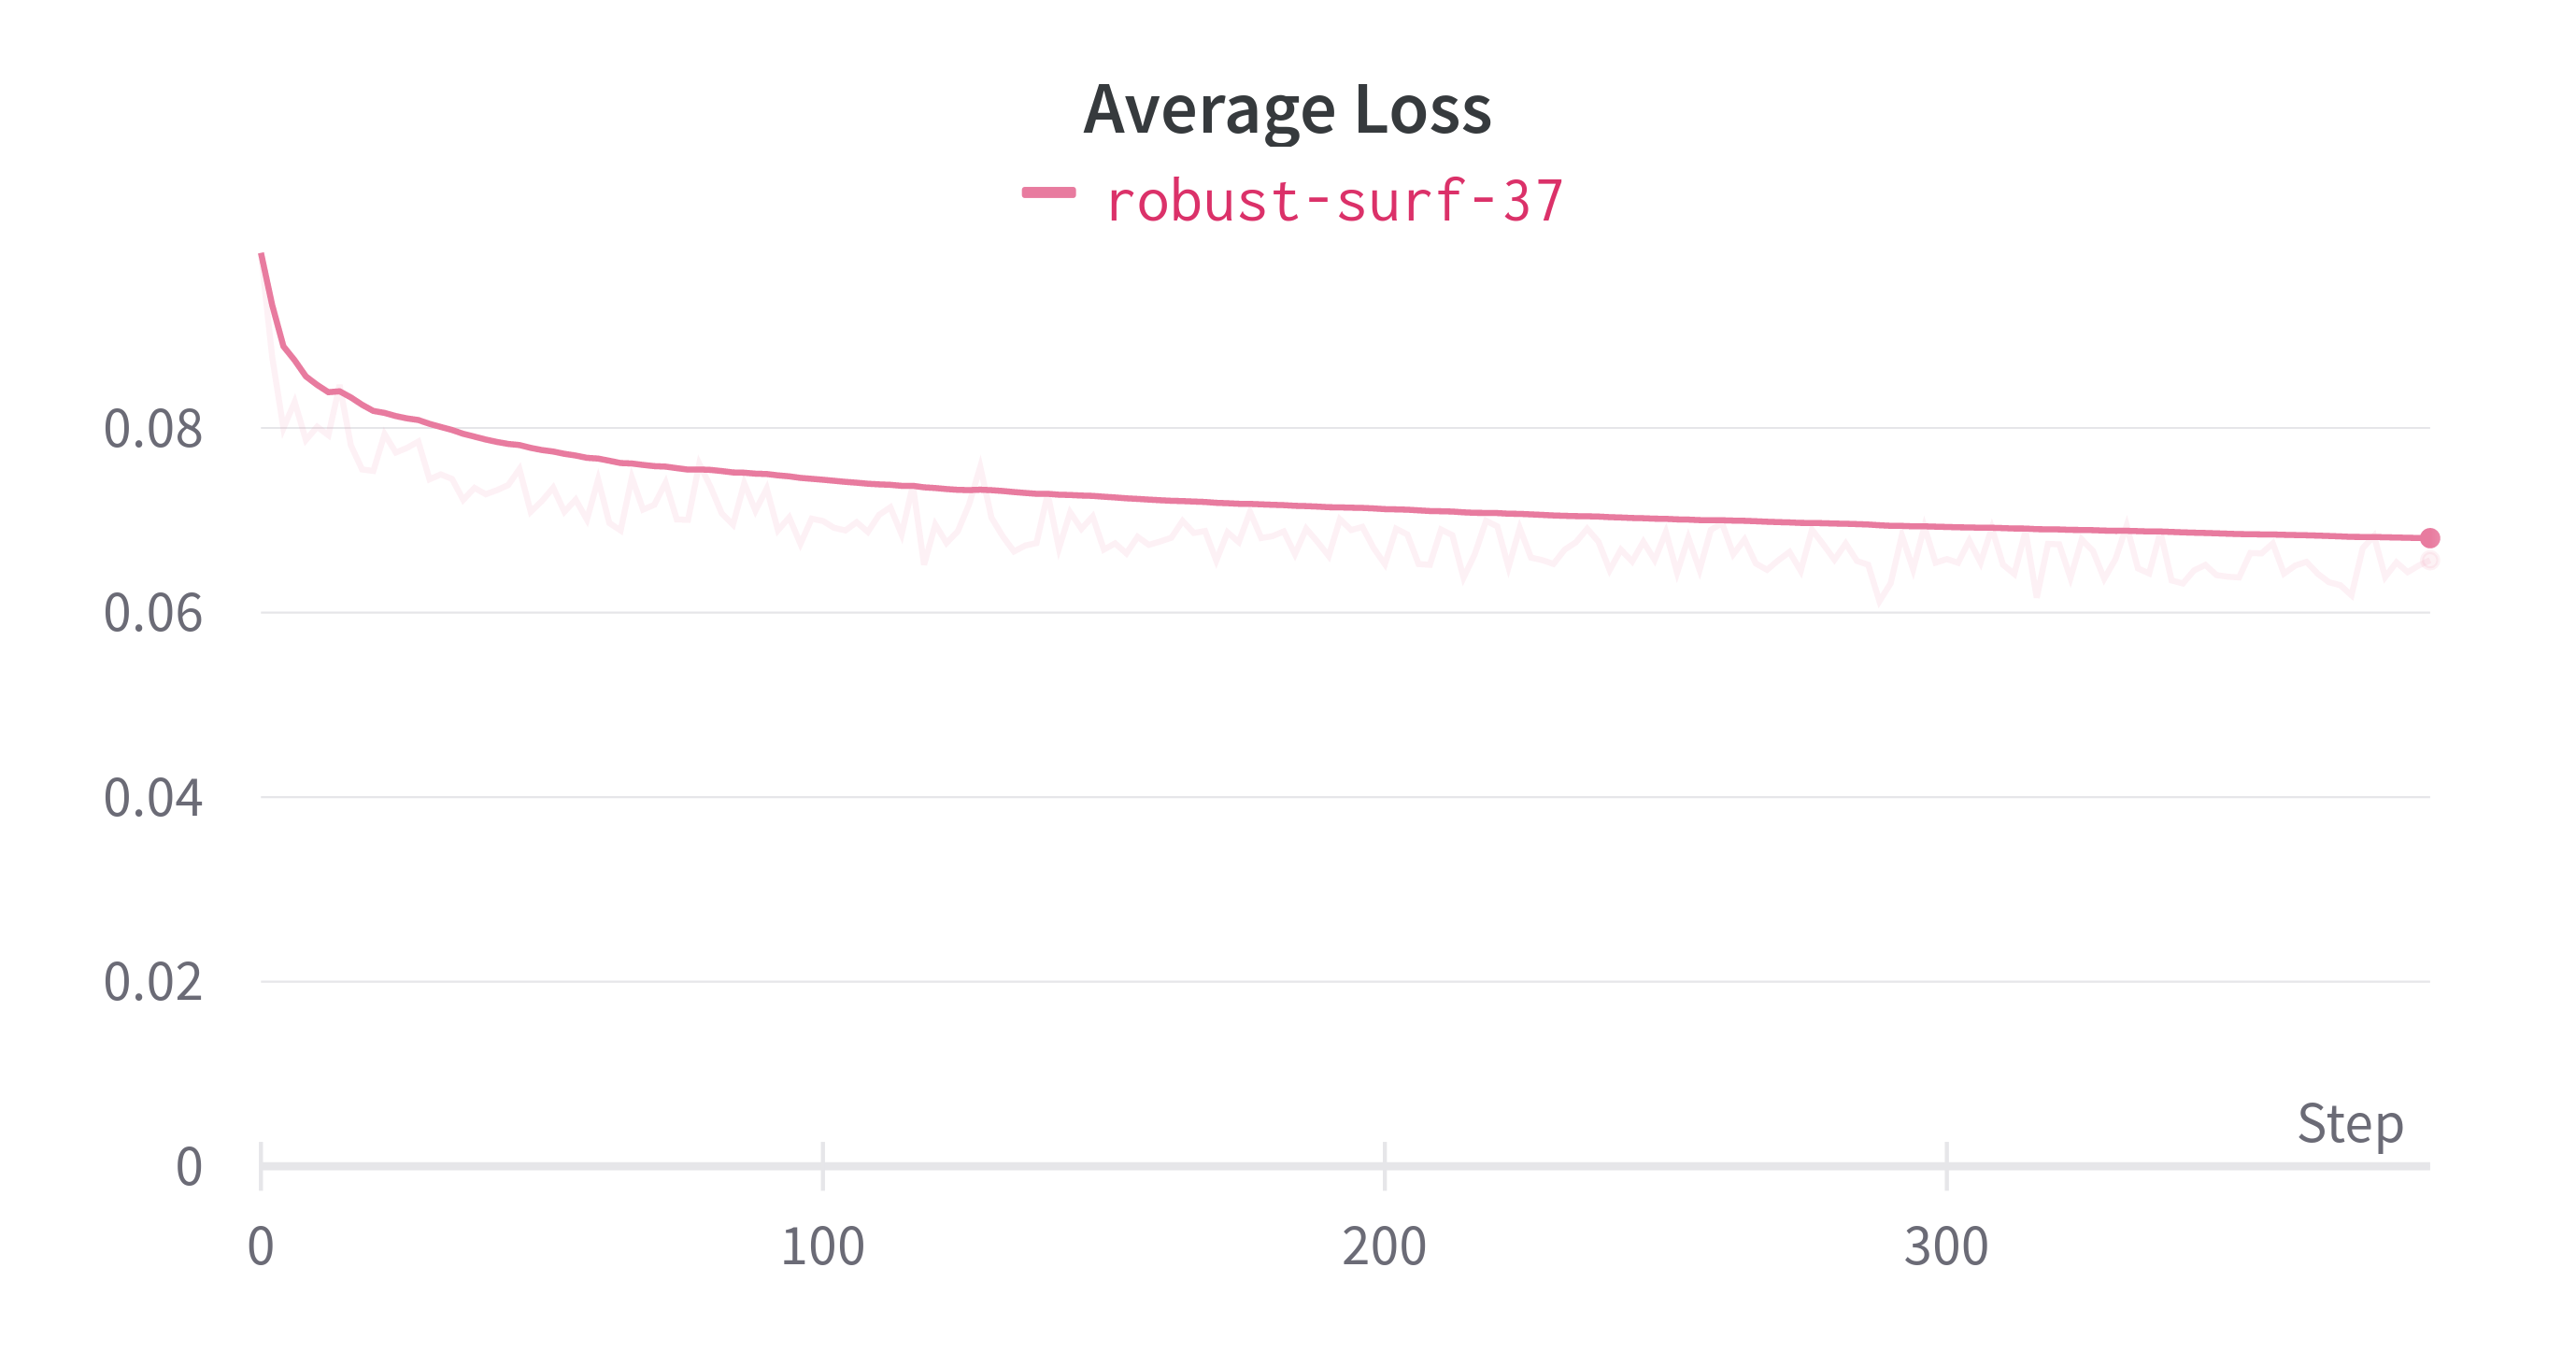
\includegraphics[width=475pt,height=275pt]{Training Loss ARU Net.png}
	\caption{Average Training Loss: ARU Net}
\end{figure}

\begin{figure}[H]
	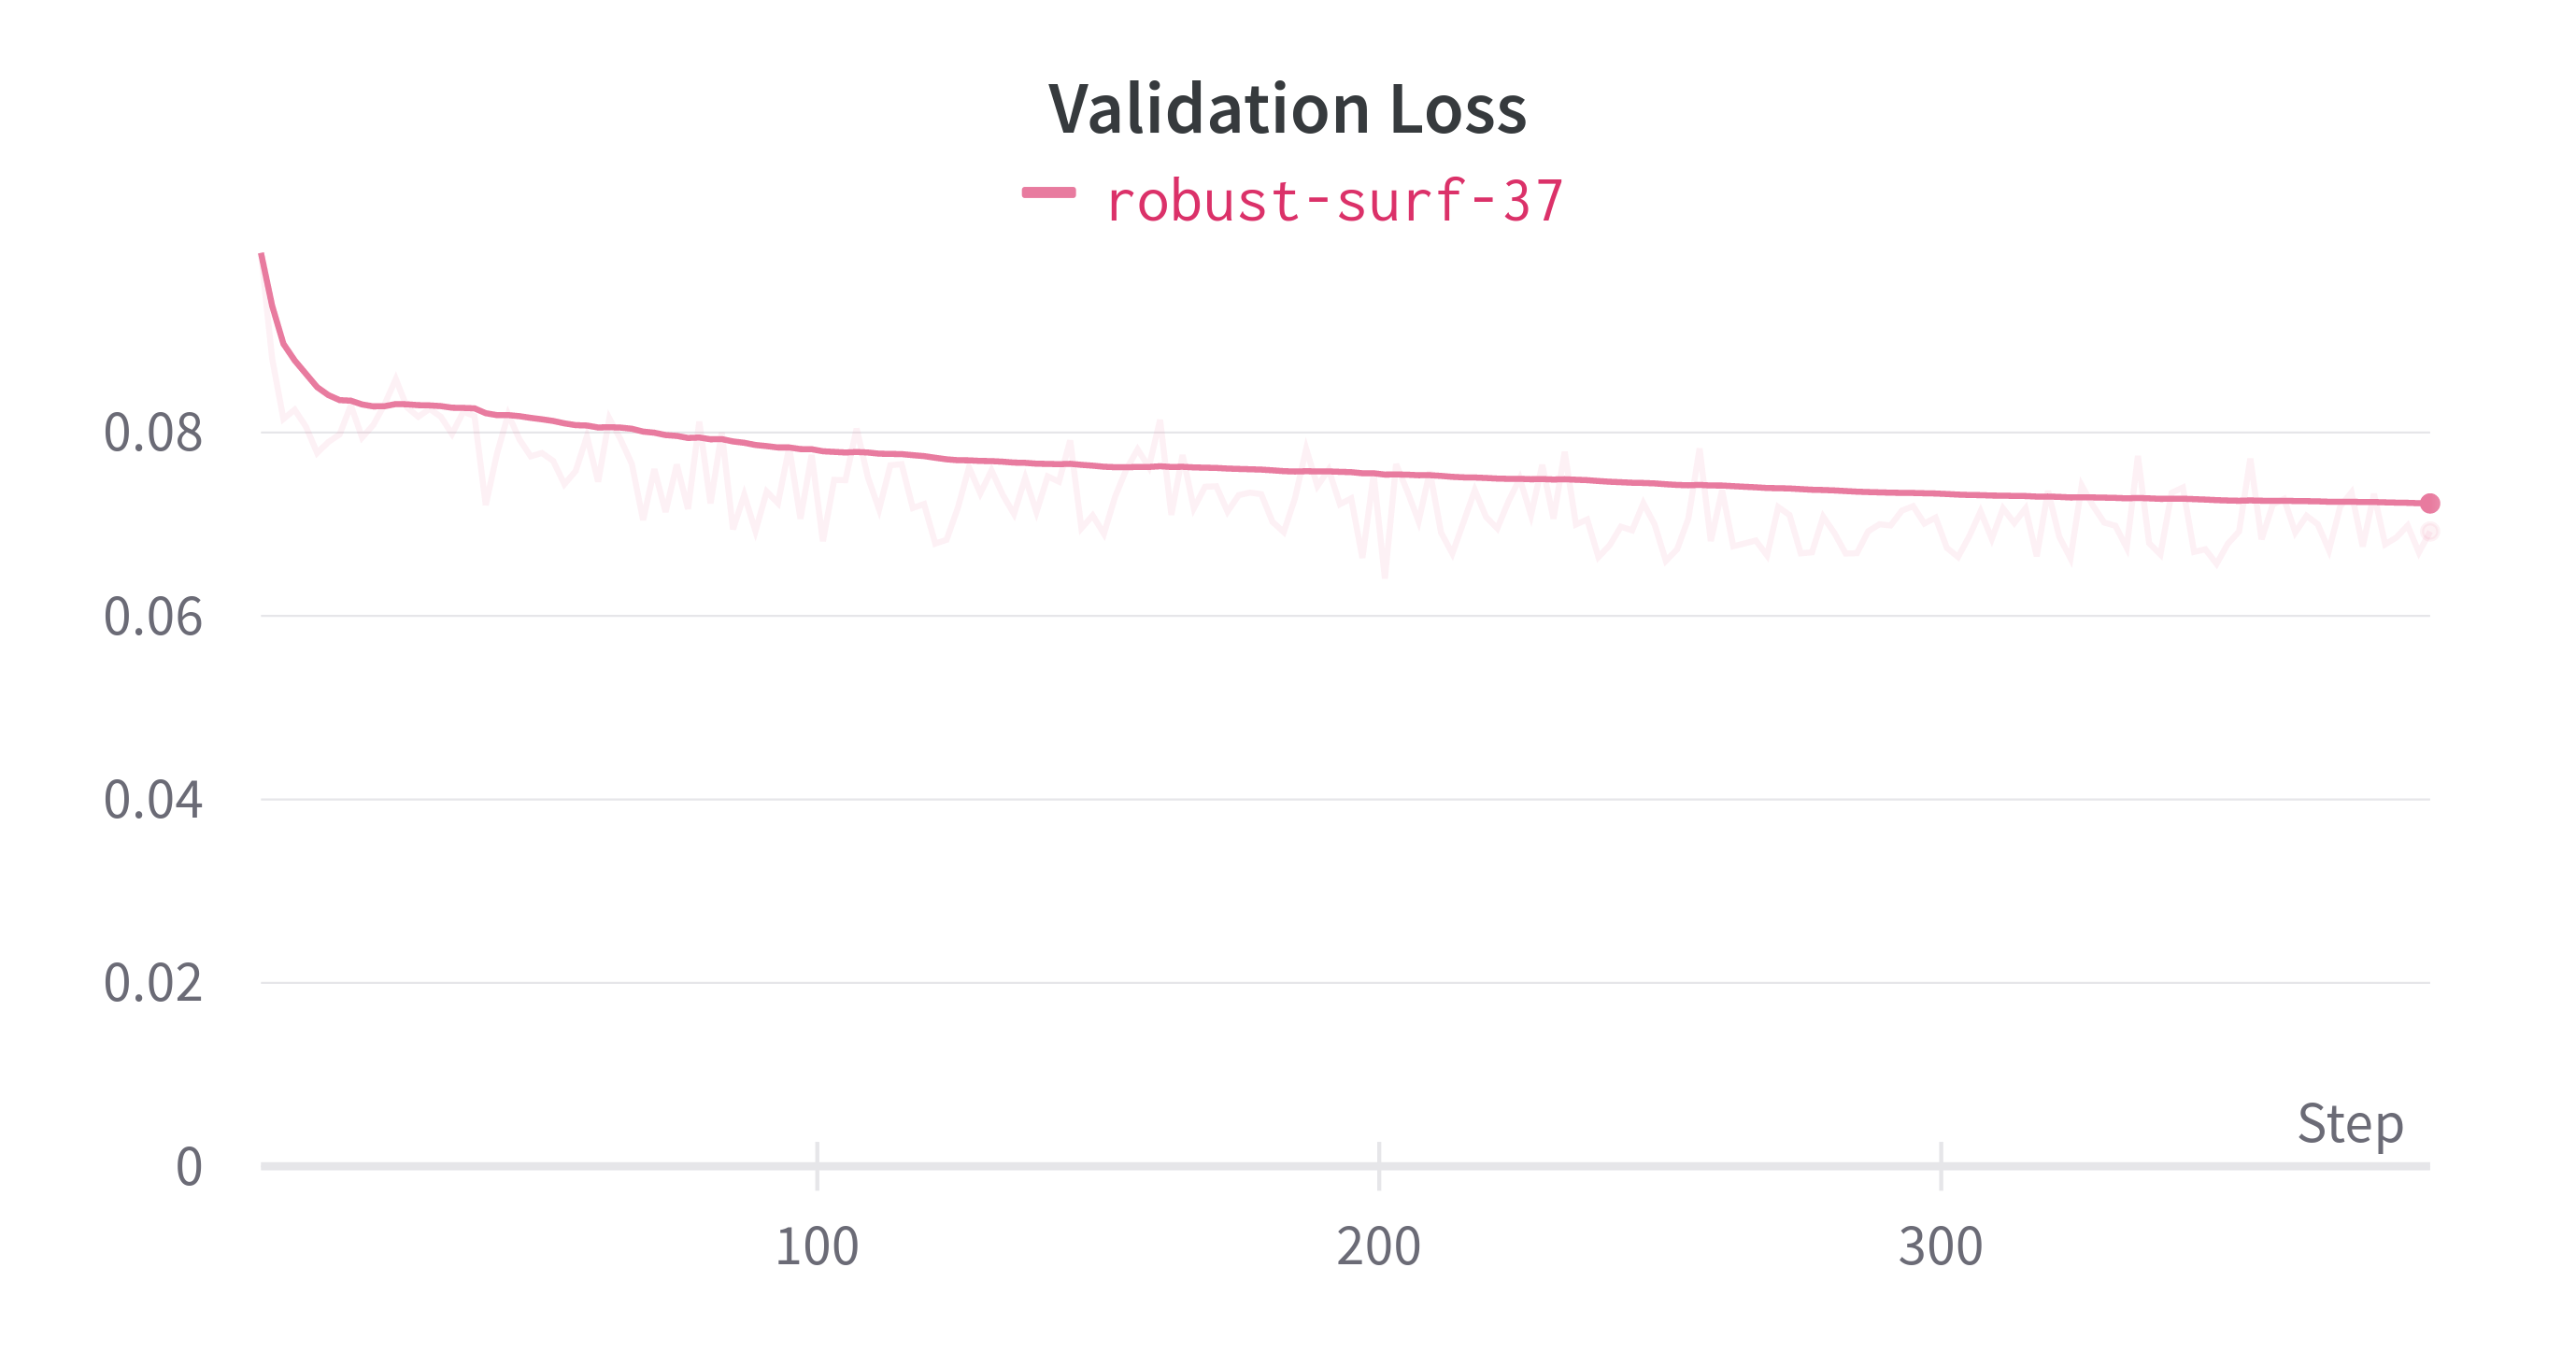
\includegraphics[width=475pt,height=275pt]{Validation Loss ARU Net.png}
	\caption{Validation Loss: ARU Net}
\end{figure}

\begin{figure}[H]
	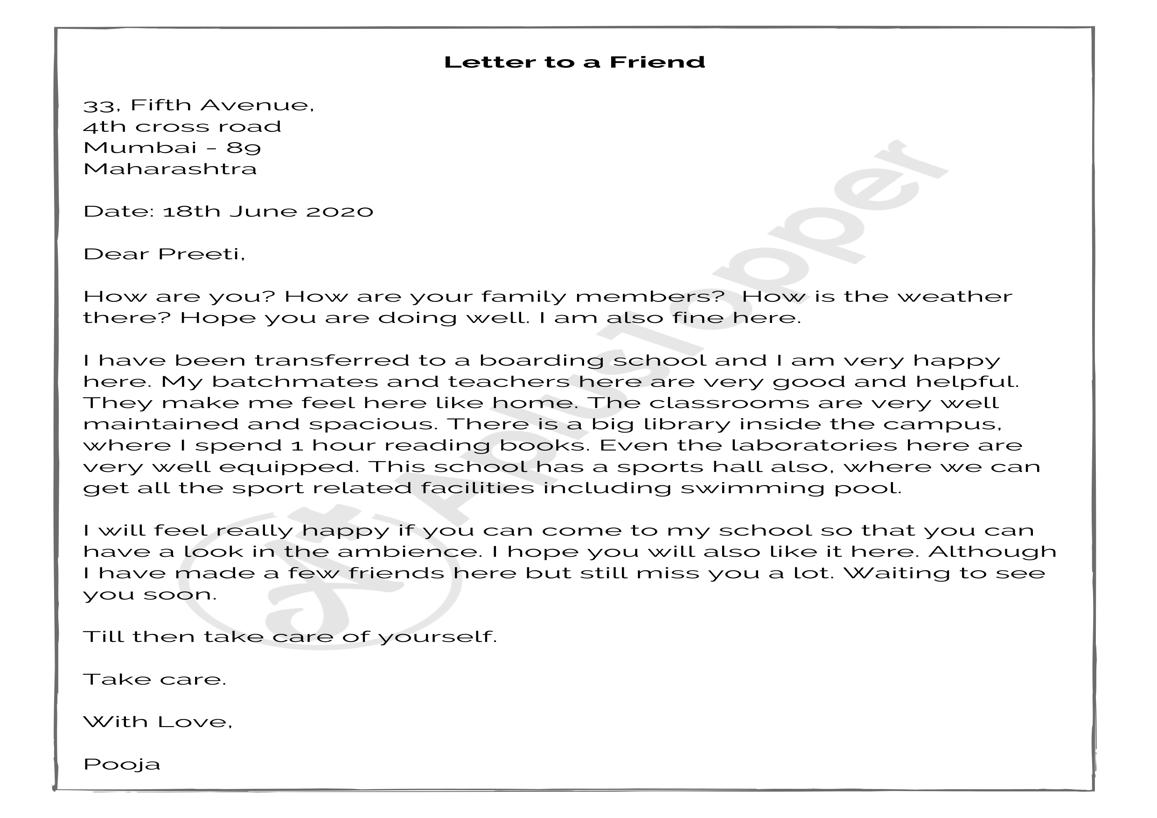
\includegraphics[width=475pt,height=275pt]{in.jpg}
	\caption{Input: ARU Net}
\end{figure}

\begin{figure}[H]
	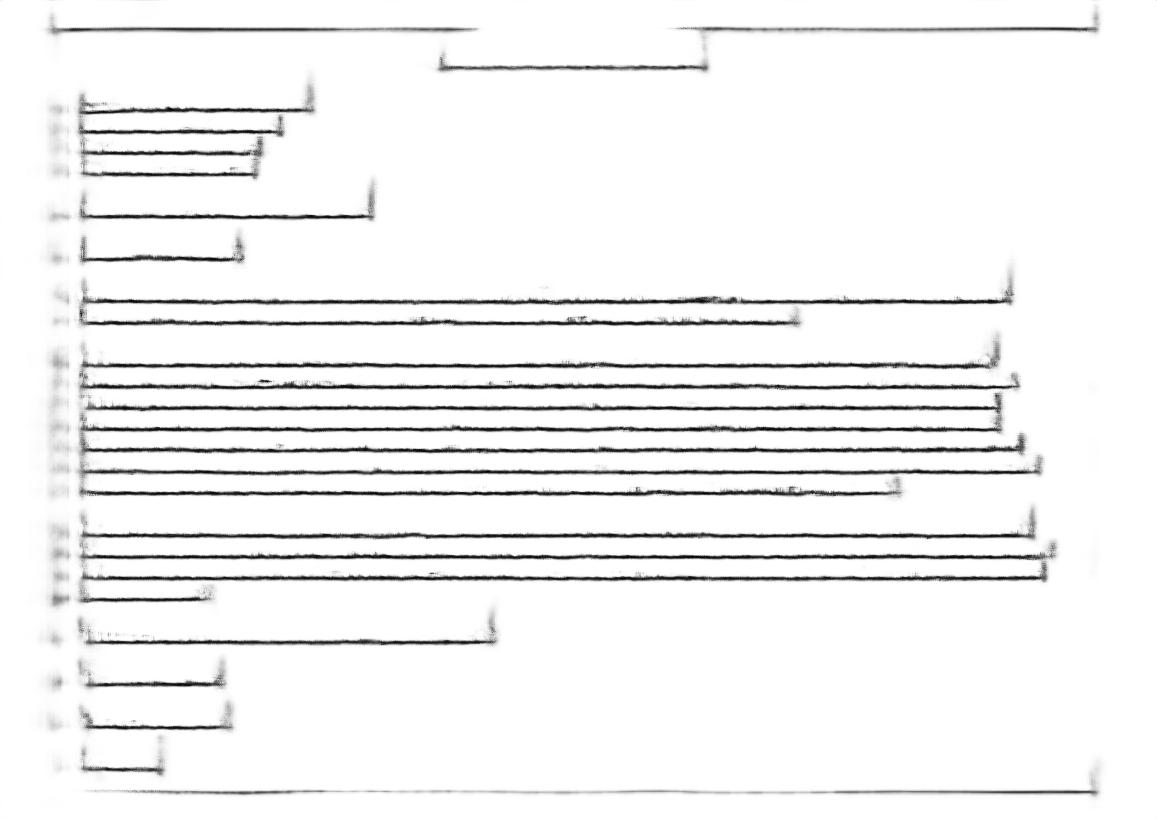
\includegraphics[width=475pt,height=275pt]{out.jpg}
	\caption{Output: ARU Net}
\end{figure}


\begin{figure}[H]
	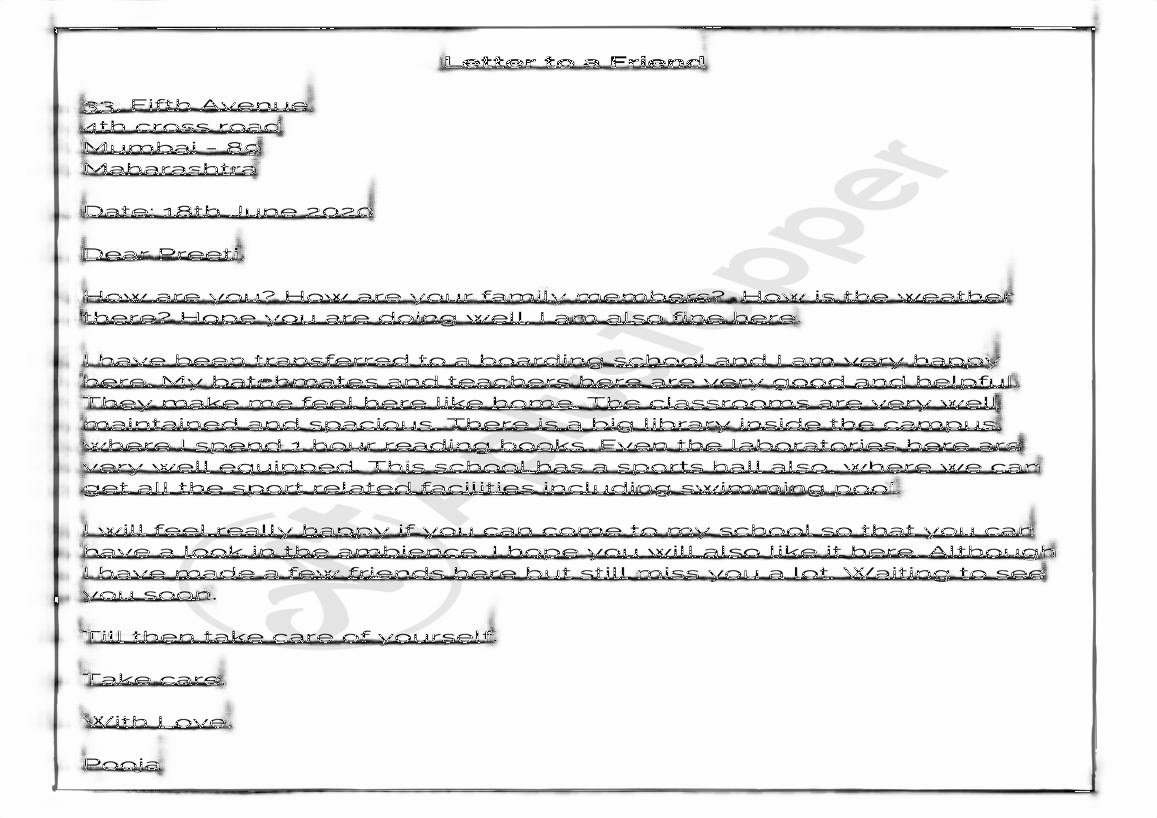
\includegraphics[width=475pt,height=275pt]{res.jpg}
	\caption{Intermediate Result: ARU Net}
\end{figure}


\begin{figure}[H]
	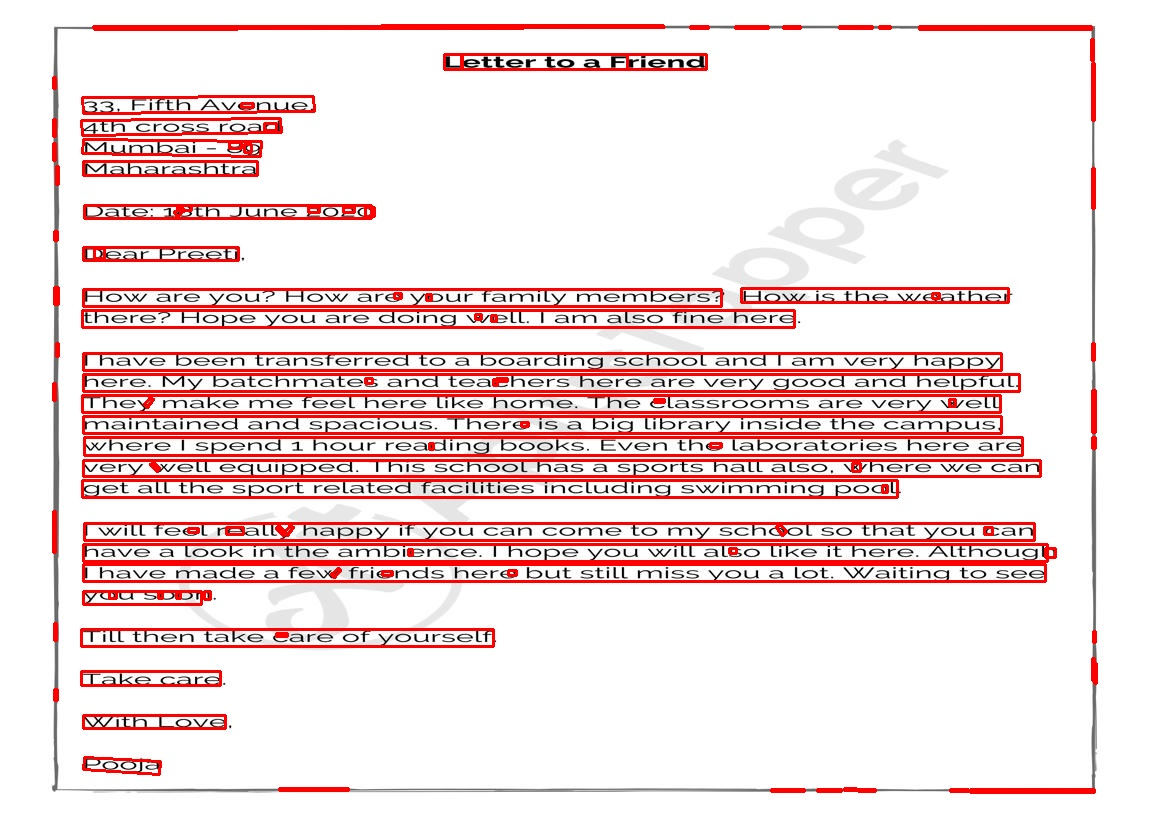
\includegraphics[width=475pt,height=275pt]{res_boxes.jpg}
	\caption{Bounding boxes: ARU Net}
\end{figure}

Shifting discussion to CRAFT network, the baseline model we started fine-tuning with, was trained on just synthetic data.Synthetic data was very different than document data where we have hundreds of words in a page as compared to just a few words in synthetic data.Also the size of the words is comparatively small as compared to synthetic dataset.The baseline model was not able to perform good on augmented documents in which text is at random angles.In all, the performance on the document data was not so great.We trained our model for around 100 epochs. An epoch takes around 90-100 minutes to complete and we analysed the results after every epoch. After certain epochs, the results start to degrade rather than improving,this can be due to the reason that the character level bounding boxes in the training data were not accurate and we were doing fully supervised learning of CRAFT.

In the first run, we didn't combine the input data with synthetic data as used by the authors and as a result, the network started to forget the past learned information and performed bad even on the examples the baseline model performed good, although the results on the handwritten documents improved a bit.

In second phase, in every batch, we combined our custom training data with synthetic data used for training the baseline model we started with,used in the ratio of 3:1 in every batch. The results of training the network with this change helped to stay good on the cases where baseline performs good as well as get better at handwritten text. There are still some issues in recognising the text in the handwritten documents in which ruling lines are present in the paper, for which the model fails to recognise the words.But the results of recognising the words on plain paper are quite good.Certain issues also exist in machine print documents where the CRAFT model fails to recognise small characters like comma,hyphens,points,single characters and it becomes extremely critical in certain business documents.The sample result images are attached here with. 

We also tuned the hyper parameters required for connected component analysis and obtaining words from region and affinity scores - link threshold, region threshold and text threshold. Region threshold filters out the pixels regions below certain value and link threshold does that for affinity scores. After combining region and affinity scores, we do connected component analysis and find a large number of components and then we use text threshold to select the appropriate components for finding the minimum area rectangles.

We have deployed the best epoch model which feeds in Word OCR model with the bounding boxes of all the words present in the page.The API is being used internally for testing. 

{\Large  \textbf{CRAFT: Graphs}}

\begin{figure}[H]
	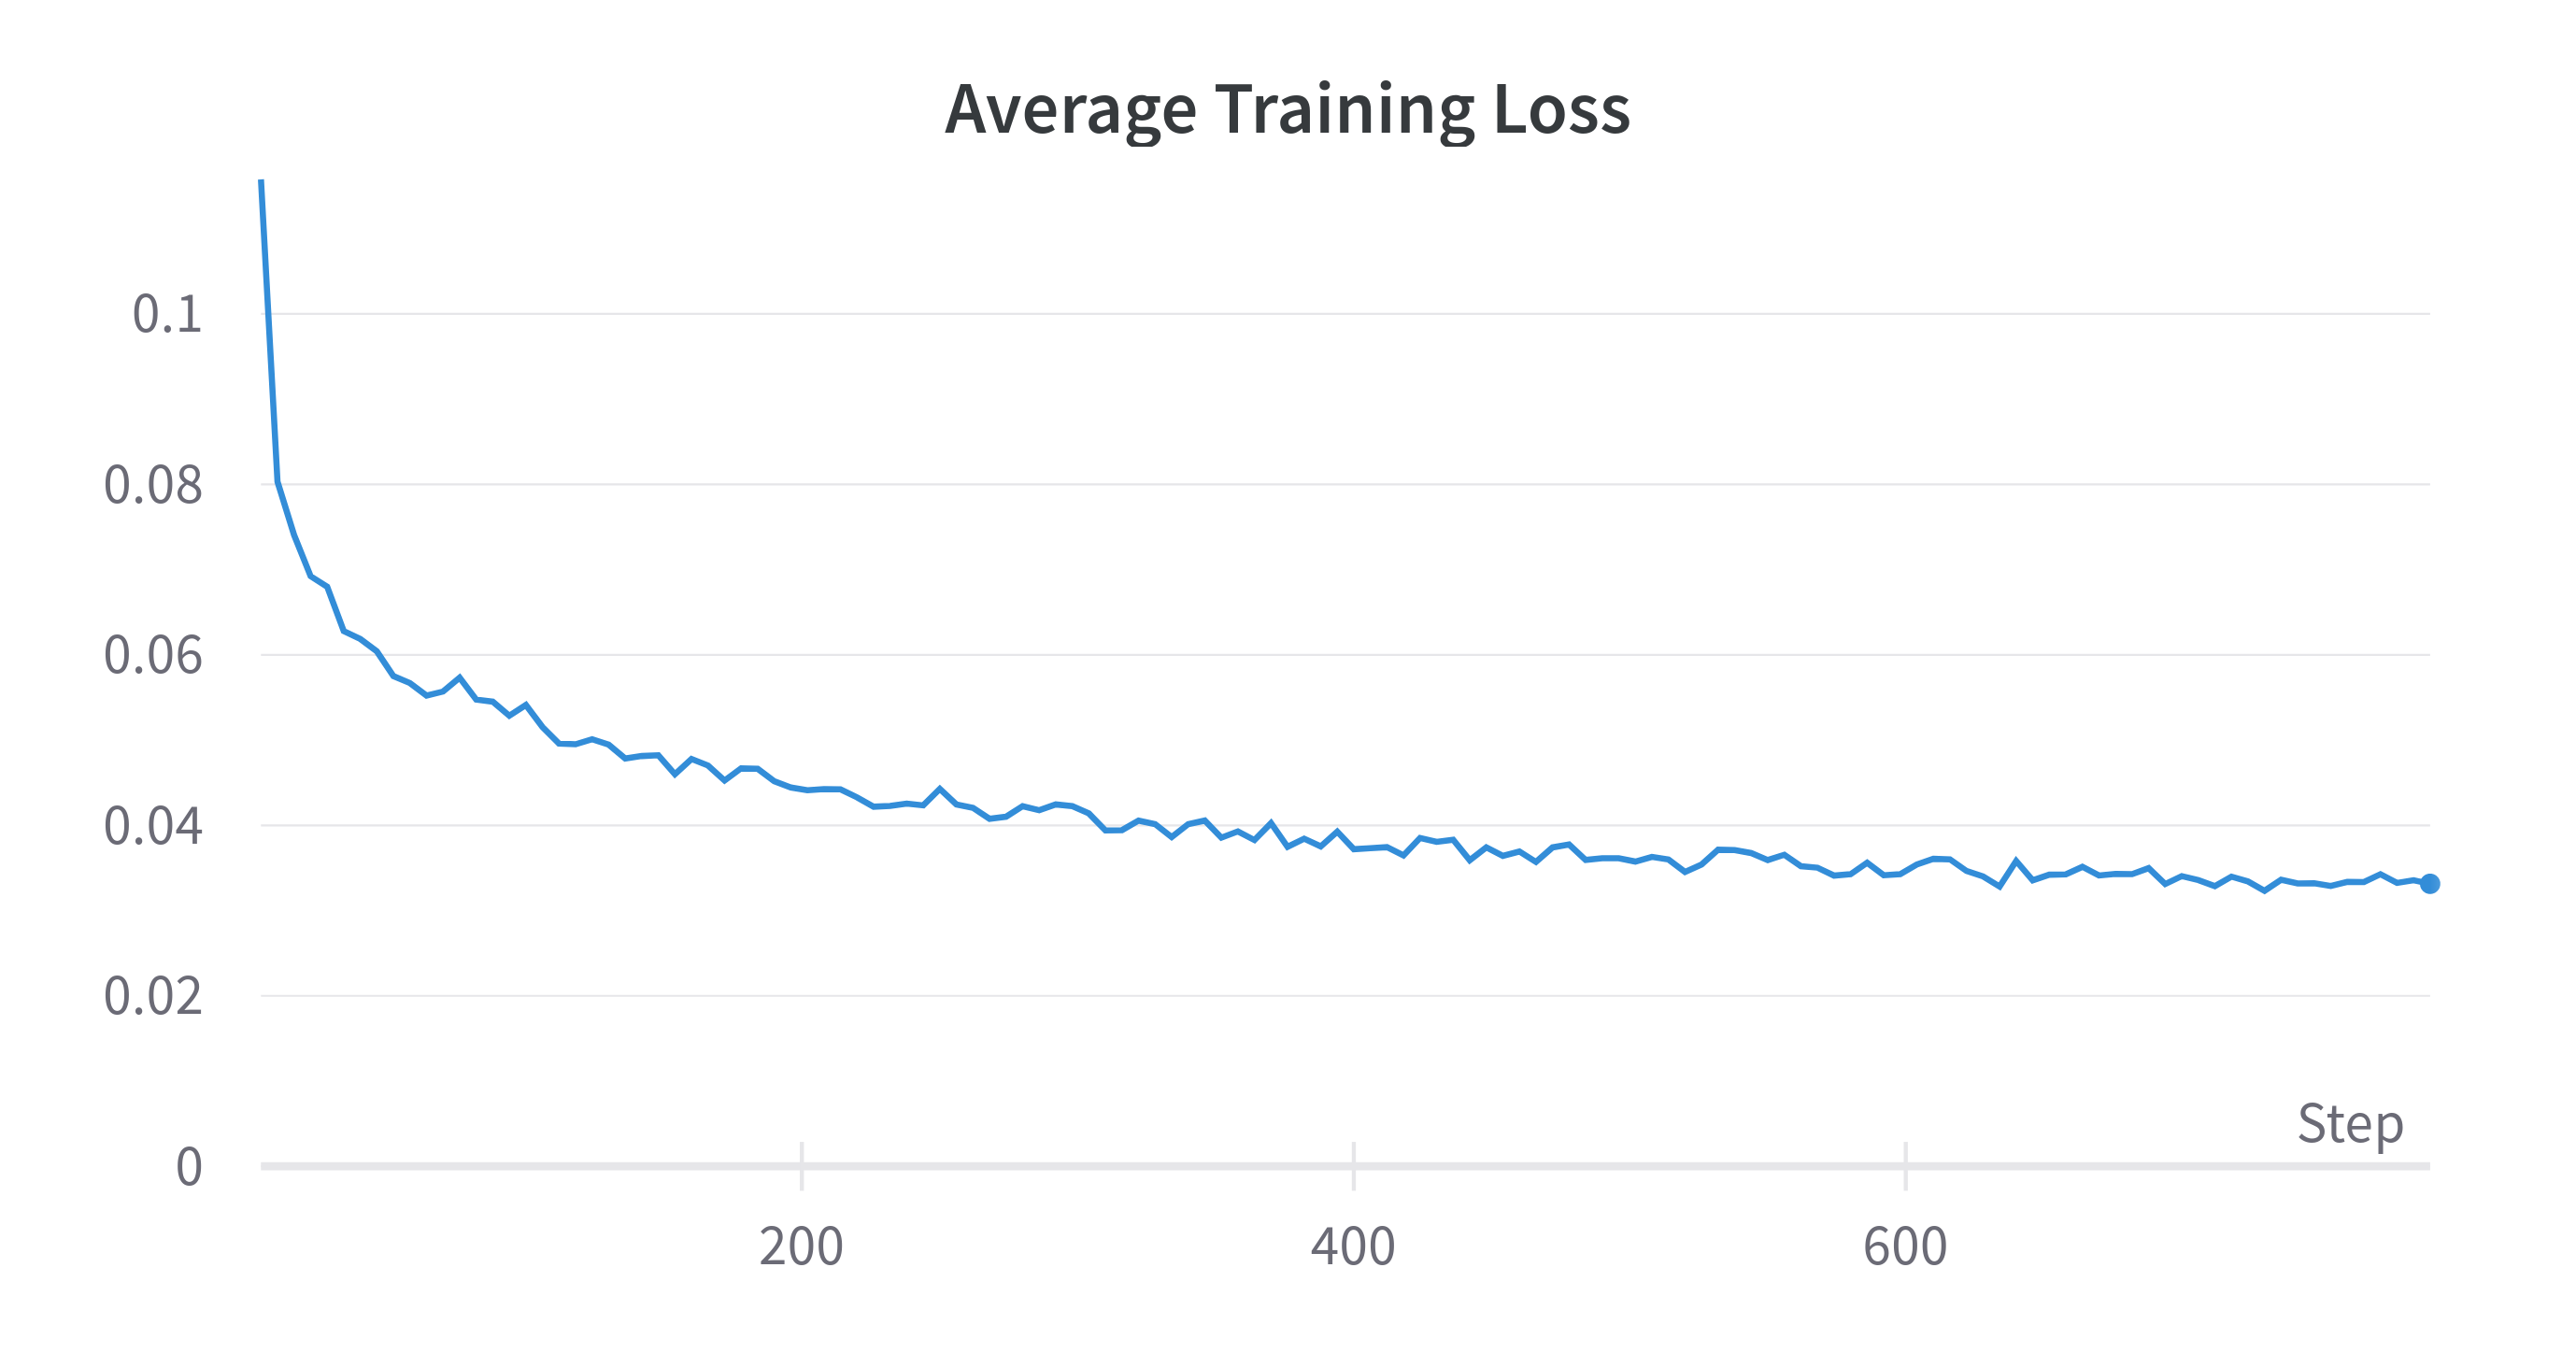
\includegraphics[width=475pt,height=275pt]{Training Loss CRAFT.png}
	\caption{Average Training Loss: CRAFT}
\end{figure}

\begin{figure}[H]
	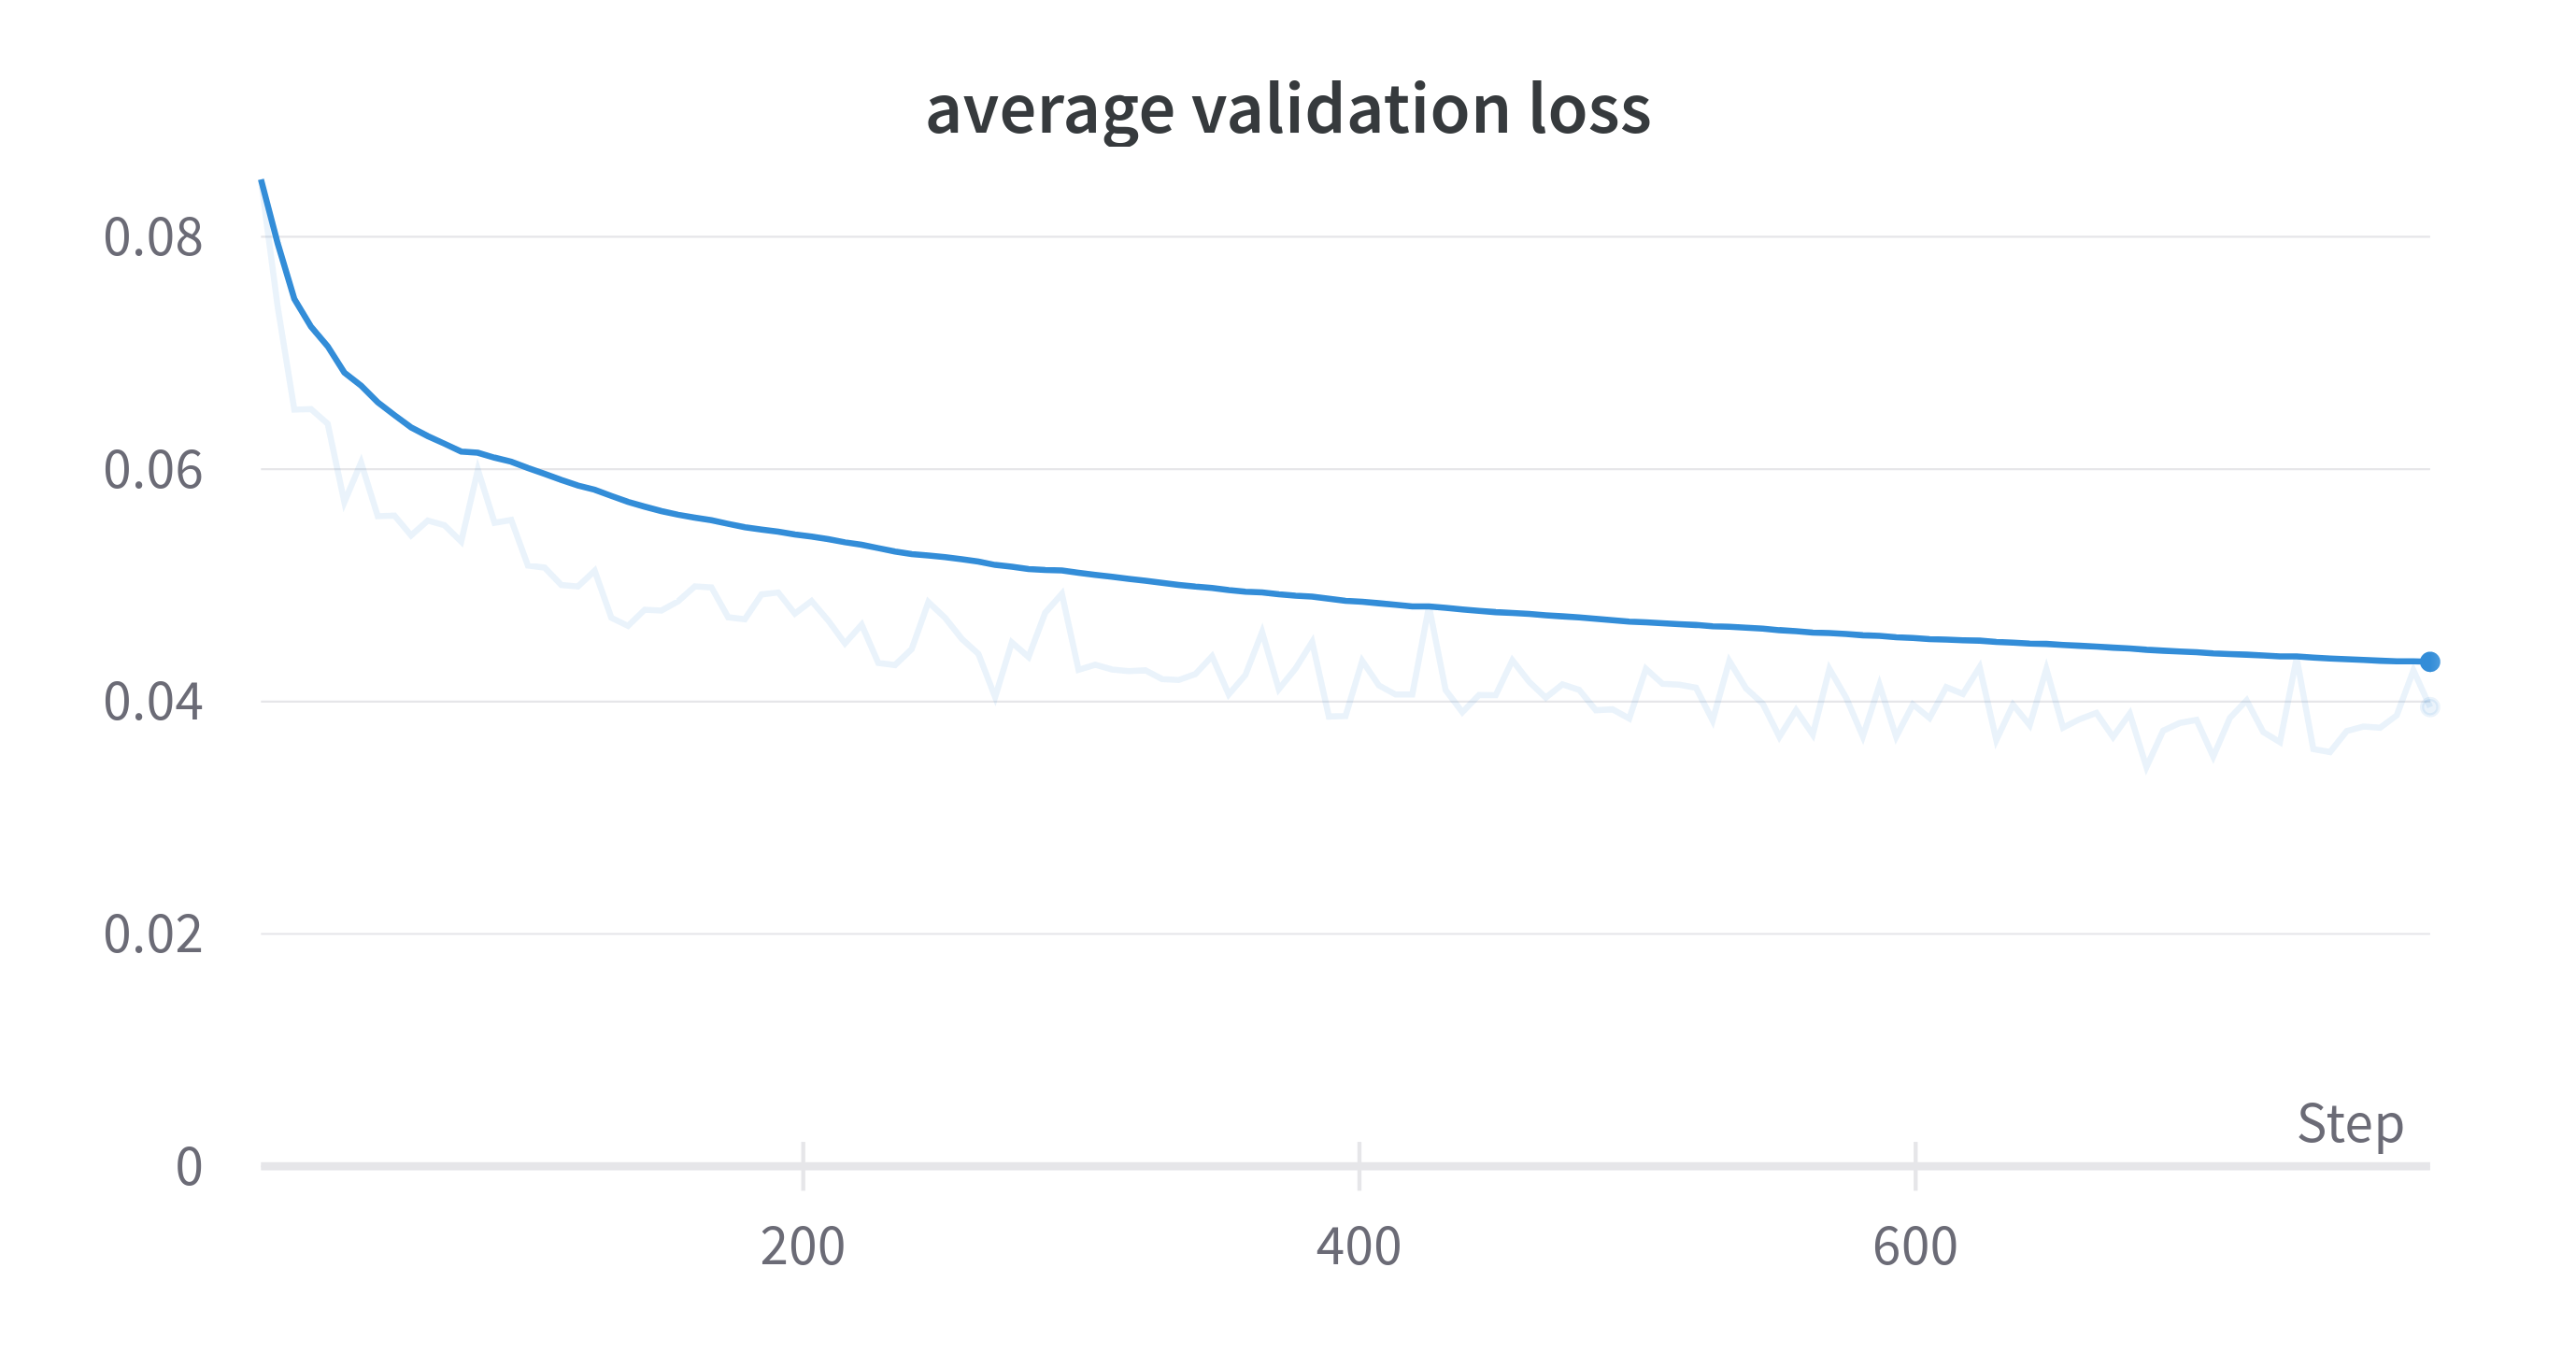
\includegraphics[width=475pt,height=275pt]{Validation Loss CRAFT.png}
	\caption{Validation Loss: CRAFT}
\end{figure}


\begin{figure}[H]
	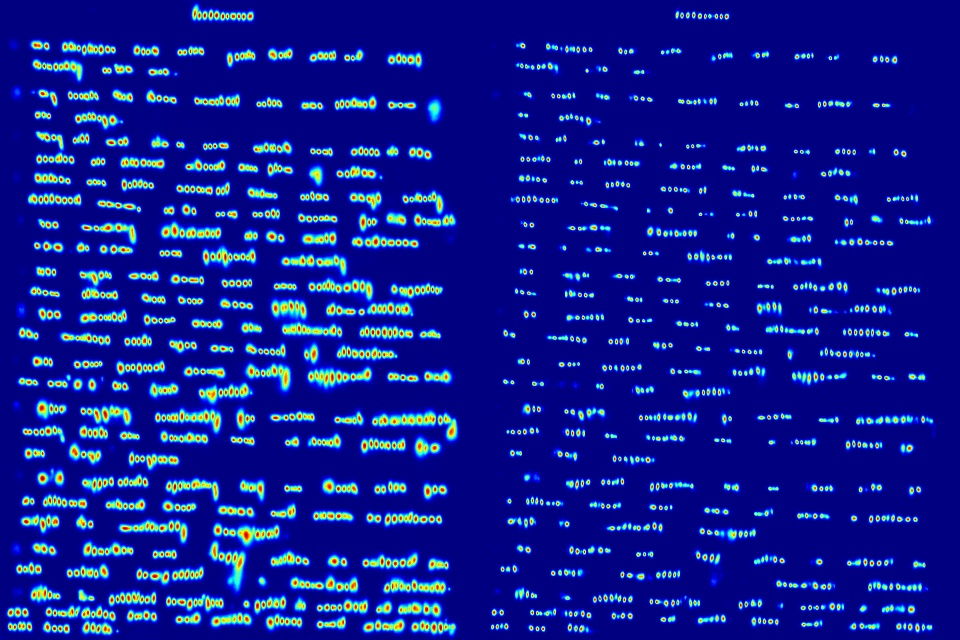
\includegraphics[width=475pt,height=275pt]{craft_mask.jpg}
	\caption{Masked output: CRAFT}
\end{figure}

\begin{figure}[H]
	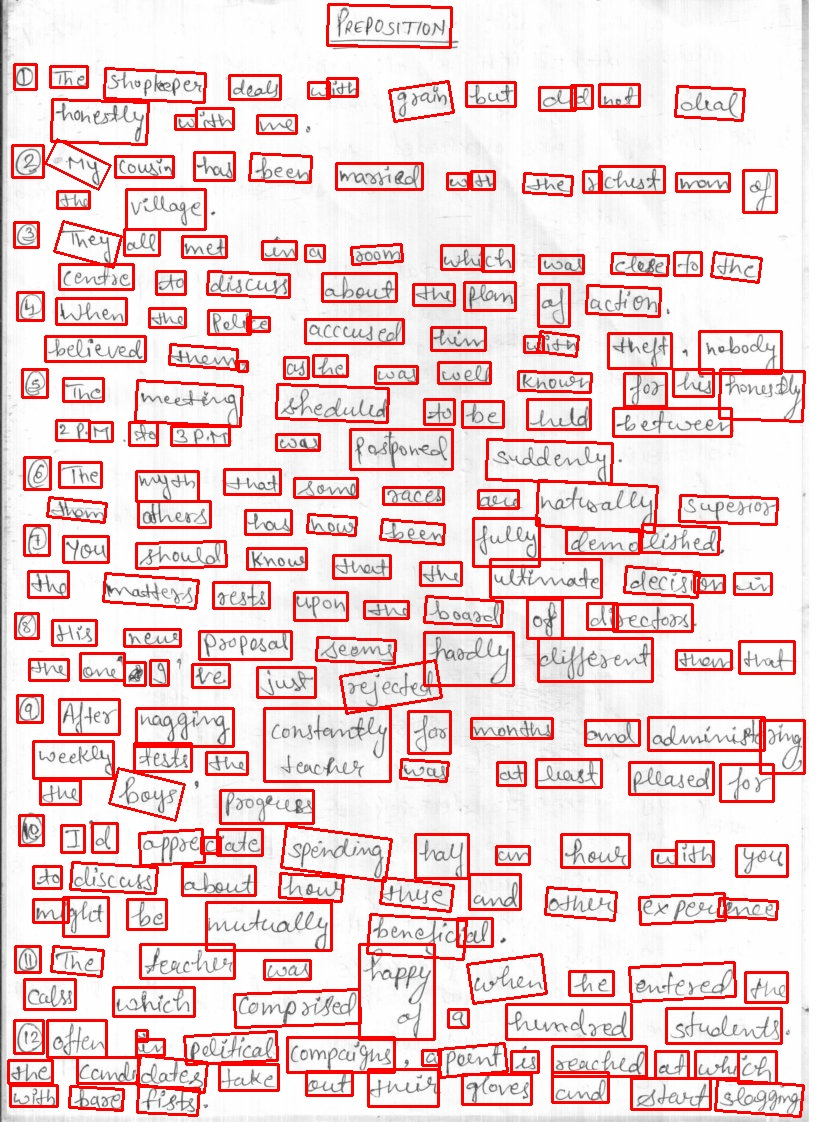
\includegraphics[width=475pt,height=275pt]{craft_out.jpg}
	\caption{Bounding Boxes: CRAFT}
\end{figure}

After introduction of word region maps, we were able to tackle the problems of word-splitting, detect missing symbols and handwritten words to a great extent.In the first iteration where we copied and opened up only last 5 convolutional layers for producing word score regions, the regions obtained did not match or even resemble the corresponding ground truth word regions that well. In the second modification,we copied the up-convolutional layers and the final convolutional layers, keeping the original up-convolutional layers frozen for computing region and affinity scores.After training the network with second modification, we were able to get a lot better word regions, looking visually very similar to the ground truth word scores.The visually improved word regions and the use of word region maps for arriving at final bounding boxes along with region and affinity maps also led to reduction in words splitting to a great extent, especially in the machine print documents.

In the post processing steps,we combined word scores with region and affinity scores and tuned various hyper parameters for obtaining word bounding boxes after doing connected component analysis.With hyper parameter adjustments, a significant improvement was also seen in detection of handwritten words.In some cases,we get no region and affinity scores but only word score regions for words in handwritten text and still we are able to detect the words after super-imposing all 3 score maps( character regions, affinity and word regions) before going through the connected component analysis followed by other post processing steps with appropriate region,affinity,word and text thresholds.For our use case, we selected text threshold as 0.3, link threshold as 0.3,region threshold as 0.4 and word threshold as 0.5.

\begin{figure}[H]
	\includegraphics[width=475pt,height=275pt]{res_image_63.jpg}
	\caption{Bounding Boxes: CRAFT on IAM image}
\end{figure}

\begin{figure}[H]
	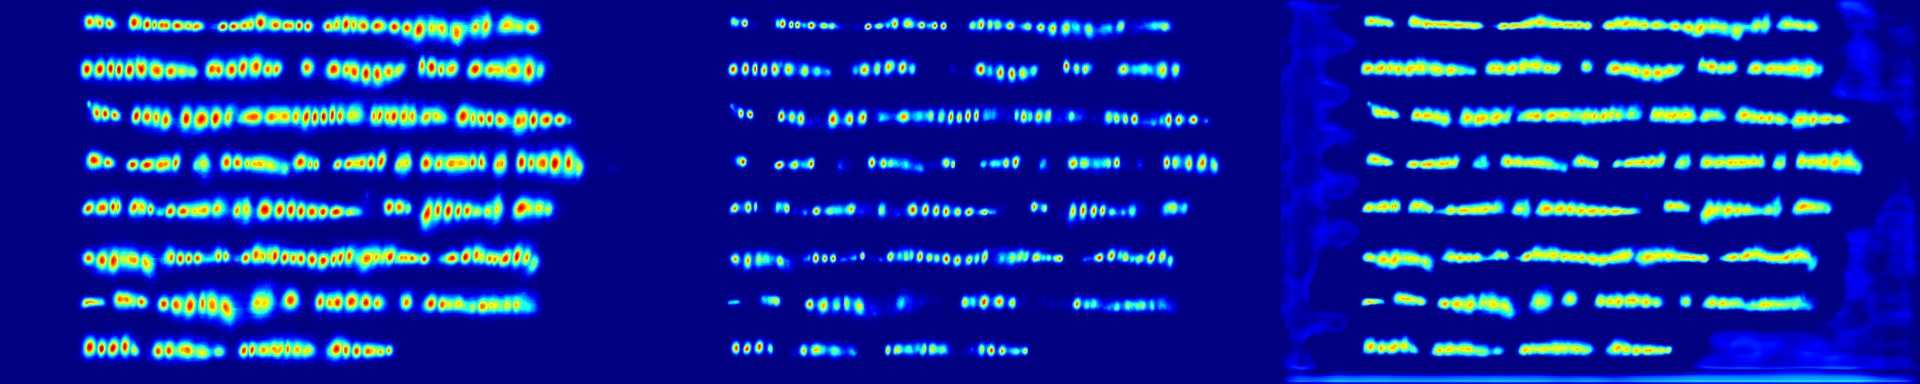
\includegraphics[width=500pt,height=235pt]{res_image_63_mask.jpg}
	\caption{Masked output: CRAFT with word scores}
\end{figure}

We prepared a custom precision and recall metric based on Intersection Over Union of detected word bounding boxes and the ground truth word boxes and used that for evaluation over a set of test images. The metric considers a detected word box as correct prediction if the IOU with the ground truth box exceeds a certain threshold. We evaluated the test set with the metric over various thresholds to know the corresponding precision and recall.


%_____________________________________________________________________________________________ 
		
%_____________________________________________________________________________________________ 
% LATEX Template: Department of Comp/IT BTech Project Reports
% Sample Chapter
% Sun Mar 27 10:25:35 IST 2011
%
% Note: Itemization, enumeration and other things not shown. A sample figure is included.
%_____________________________________________________________________________________________ 

\setstretch{1.5}
{\let\clearpage\relax \chapter{Conclusion}}

We started out with the goal of getting better at text recognition, focusing on handwritten text and identified 3 paths - text segmentation, improving image quality and doing character level segmentation and recognition. We started on the path of text segmentation and tried 2 networks - ARU Net and CRAFT. As discussed in the results section, ARU Net just gives use the baselines and we heavily depend on our post processing techniques to reach the text segmentation we want. This approach does a descent job in identifying the lines but there are certain cases, still not addressed,  regarding mis predictions in case of complex handwritten data and irregular number of boxes for a line in case of machine print images.For CRAFT, using supervised learning, we weren't able to reach some good results since its difficult to gather character level bounding box data for handwritten documents and the dataset we used, also had several inaccurate character level bounding boxes. We got better at recognising the handwritten text while continuing doing good on machine print document,but the model is not enough good as of now to be production ready.

\textbf{Ongoing Experiments and future scope:} We are exploring the path of semi-supervised learning to get better at segmentation using CRAFT where in we provide the word level bounding boxes and let the the network figure out the character level regions using the interm model trained on synthetic data. Several experiments are also being done for training the model in shorter time, using multuple dataloaders, parallel processing and maximising the GPU usage.We are also planning to work on improving the handwritten OCR model so as to get better at recognising handwriting after segmentation.Some optimisations in the post processing techniques are also underway to get better text recognition results.We have also planned certain changes to original CRAFT implementation in terms of changing the network architecture to do transfer learning to get to the kind of model outputs that help us more in post processing.All such experiments are being worked on. 

%_____________________________________________________________________________________________ 
		
		

\appendix

\bibliographystyle{plain}  	  % You can ch\textsc{}ange the style of writing bibliography.
{\let\clearpage\relax \bibliography{bib.bib}} % Instead of a .bib file, you can just write it in 

				  % a text file with \bibitem entries.
%_____________________________________________________________________________________________ 
\end{document}			% End of Report
